\section{Auswertung}
\label{sec:Auswertung}

Nach der Messung werden die Filmstreifen ausgemessen. Dies geschieht aufgrund von fehlenden Werkzeugen mit einem gemeinen Lineal. Der systematische Fehler wird dabei auf $\pm\SI{1}{mm}$ gesetzt. Gemessen wird der Abstand zwischen zwei Linien, also der Kegelradius. Der Abstand zwischen dem Eintritts- und dem Austrittsloch beträgt \SI{180}{mm} und deckt einen Winkel $\pi$ der Kammer ab. Wie in Abbildung \ref{fig:sys2} zu sehen ist, wird in einer Hälfte der Kammer zwischen Eintritts- und Austrittsloch ein Winkel von $2\theta$ abgedeckt. Daraus lässt sich $\theta$ mit Gleichung (\ref{eqn:theta}) berechnen.
\begin{equation}
\label{eqn:theta}
	2\theta = x \cdot \frac{\pi}{\SI{180}{mm}} \Longrightarrow \theta = x \cdot \frac{\pi}{\SI{360}{mm}}
\end{equation}
Hierbei ist $x$ der Kegelradius. In Tabelle \ref{tab:KegelMetall} sind die gemessenen Kegelradien und die zugehörigen Winkel für Metall zu sehen. In Tabelle \ref{tab:KegelSalz} entsprechendes für Salz.
%
% \begin{table}[h]
% \centering
% \caption{Kegelradien gemessen an den Filmstreifen umgerechnet in den Winkel $\theta$ für Metall.}
% \label{tab:Kegel}
% 	\begin{minipage}[t]{0.4\textwidth}
% 	% \begin{table}[h]
% 	% \centering
% 	\caption{}
% 	\label{tab:KegelMetall}
% 	\begin{tabular}{c | c}
% 			\hline
% 			\text{Kegelradius $x$ [mm]} & \text{Winkel $\theta$} \\
% 			\hline
% 			44.5\pm1 &  0.388\pm0.009 \\
% 			64.5\pm1 &  0.563\pm0.009 \\
% 			81.5\pm1 &  0.711\pm0.009 \\
% 			98.5\pm1 &  0.860\pm0.009 \\
% 			114.5\pm1 & 0.999\pm0.009 \\
% 			134.5\pm1 & 1.174\pm0.009 \\
% 			\hline
% 	\end{tabular}
% 	% \end{table}
% 	\end{minipage}
% 	%
% 	\begin{minipage}[t]{0.4\textwidth}
% 	% \begin{table}[h]
% 	% \centering
% 	\caption{}
% 	\label{tab:KegelSalz}
% 	\begin{tabular}{c | c}
% 			\hline
% 			\text{Kegelradius $x$ [mm]} & \text{Winkel $\theta$} \\
% 			\hline
% 			23\pm1 & 0.240\pm0.009 \\
% 			34.5\pm1 & 0.340\pm0.009 \\
% 			43\pm1 & 0.415\pm0.009 \\
% 			51\pm1 & 0.484\pm0.009 \\
% 			57\pm1 & 0.537\pm0.009 \\
% 			65\pm1 & 0.607\pm0.009 \\
% 			78\pm1 & 0.720\pm0.009 \\
% 			83\pm1 & 0.764\pm0.009 \\
% 			90\pm1 & 0.825\pm0.009 \\
% 			95.5\pm1 & 0.873\pm0.009 \\
% 			103\pm1 & 0.938\pm0.009 \\
% 			108\pm1 & 0.982\pm0.009 \\
% 			116\pm1 & 1.052\pm0.009 \\
% 			133\pm1 & 1.200\pm0.009 \\
% 			\hline
% 	\end{tabular}
% 	% \end{table}
% 	\end{minipage}
% \end{table}
%
\begin{table}[h]
\centering
\caption{Kegelradien gemessen an den Filmstreifen umgerechnet in den Winkel $\theta$ für Metall.}
\label{tab:KegelMetall}
\begin{tabular}{c | c}
		\hline
		\text{Kegelradius $x$ [mm]} & \text{Winkel $\theta$} \\
		\hline
		44.5\pm1 &  0.388\pm0.009 \\
		64.5\pm1 &  0.563\pm0.009 \\
		81.5\pm1 &  0.711\pm0.009 \\
		98.5\pm1 &  0.860\pm0.009 \\
		114.5\pm1 & 0.999\pm0.009 \\
		134.5\pm1 & 1.174\pm0.009 \\
		\hline
\end{tabular}
\end{table}
\begin{table}[h]
\centering
\caption{Kegelradien gemessen an den Filmstreifen umgerechnet in den Winkel $\theta$ für Salz.}
\label{tab:KegelSalz}
\begin{tabular}{c | c}
		\hline
		\text{Kegelradius $x$ [mm]} & \text{Winkel $\theta$} \\
		\hline
		27.5\pm1 & 0.240\pm0.009 \\
		39.0\pm1 & 0.340\pm0.009 \\
		47.5\pm1 & 0.415\pm0.009 \\
		55.5\pm1 & 0.484\pm0.009 \\
		61.5\pm1 & 0.537\pm0.009 \\
		69.5\pm1 & 0.607\pm0.009 \\
		82.5\pm1 & 0.720\pm0.009 \\
		87.5\pm1 & 0.764\pm0.009 \\
		94.5\pm1 & 0.825\pm0.009 \\
		100.0\pm1 & 0.873\pm0.009 \\
		107.5\pm1 & 0.938\pm0.009 \\
		112.5\pm1 & 0.982\pm0.009 \\
		120.5\pm1 & 1.052\pm0.009 \\
		137.5\pm1 & 1.200\pm0.009 \\
		\hline
\end{tabular}
\end{table}
Für spätere Berechnungen wird außerdem der Netzebenenabstand $d$ benötigt.
\begin{equation}
\label{eqn:d}
	d = \frac{\lambda}{2\sin(\theta)}
\end{equation}

\subsection{Nicht verschwindende Reflexe}

Mit den bestimmten Winkeln und Gleichung (\ref{eq:Struk2}) kann nun die Strukturamplitude für verschiedene Netzebenen und damit verschiedene $[hkl]$-Werte bestimmt werden. Genau genommen ist für die Bestimmung der nicht verschwindenden Reflexe nur interessant ob $S(hkl)$ verschwindet oder nicht. In Tabelle \ref{tab:Strukturen} sind für die kubischen Gitter (SC, BCC, FCC und Diamant) die ersten sechs, laut Theorie, nicht verschwindenden Reflexe.
%
\begin{table}[h]
\centering
\caption{Es sind für die kubischen Gitter (SC, BCC, FCC und Diamant) die ersten sechs, laut Theorie, nicht verschwindenden Reflexe dargestellt.}
\label{tab:Strukturen}
\begin{tabular}{c | c | c | c}
		\hline
		SC & BCC & FCC & Diamant \\
		\hline
		100 & 110 & 111 & 111 \\
		110 & 200 & 200 & 220 \\
		111 & 211 & 220 & 311 \\
		200 & 220 & 311 & 400 \\
		210 & 310 & 222 & 331 \\
		211 & 222 & 400 & 422 \\
		\hline
\end{tabular}
\end{table}

Für die Strukturbestimmung des Salzes (Zinkblende-, Steinsalz-, Caesiumchlorid- und Fluoritstruktur) müssen die Formfaktoren in Gleichung (\ref{eq:Struk2}) berücksichtigt werden. Deswegen kann nicht bestimmt werden ob die Reflexe verschwinden, sondern nur die Intensität der Linien.

\subsection{Bestimmung der Kristallstruktur}

Aus Gleichung (\ref{eq:Abstand4}) und (\ref{eqn:d}) folgt
\begin{equation*}
	d = \frac{a}{\sqrt{h^2 + k ^2 + l^2}} = \frac{a}{m} = \frac{\lambda}{2\sin(\theta)} \text{ mit }m\equiv\sqrt{h^2 + k ^2 + l^2}.
\end{equation*}
Damit lässt jedes $m$ auf den ersten nicht verschwindenden Reflex normieren und mit den experimentell bestimmten Werten vergleichen:
\begin{equation*}
	\frac{m_i}{m_1} = \frac{\sin{\theta_i}}{\sin{\theta_1}}.
\end{equation*}
Durch den Vergleich von Daten und Theorie wird die Struktur bestimmt. In Abbildung \ref{fig:verhaeltnisse} ist die Übereinstimmung der Verhältnisse jeweils für Metall und Salz zu sehen. Des weiteren wird die Abweichung der Daten von der Theorie bestimmt durch
\begin{equation*}
	\Chi^2 = \sum\frac{\left(\frac{\sin{\theta_i}}{\sin{\theta_1}} - \frac{m_i}{m_1}\right)^2}{\frac{m_i}{m_1}}.
\end{equation*}
Wie bereits in Abbildung \ref{fig:verhaeltnisse_metall} zu sehen ist, lässt sich das SC- und das BCC-Gitter für Metall mit so wenigen Daten nicht unterscheiden. Die Werte für alle Gitter sind in Tabelle \ref{tab:Xi} zu sehen.
%
\begin{table}[h]
\centering
\caption{Es sind für die kubischen Gitter (SC, BCC, FCC und Diamant) die $\Chi^2$ dargestellt.}
\label{tab:Xi}
\begin{tabular}{c | c | c | c | c}
		\hline
		& SC & BCC & FCC & Diamant \\
		\hline
		$\Chi^2$ & $0.0002\pm0.0018$ & $0.0002\pm0.0018$ & $0.10\pm0.04$ & $0.18\pm0.05$ \\
		\hline
\end{tabular}
\end{table}
%
\begin{figure}[h]
	\begin{minipage}[t]{0.45\textwidth}
		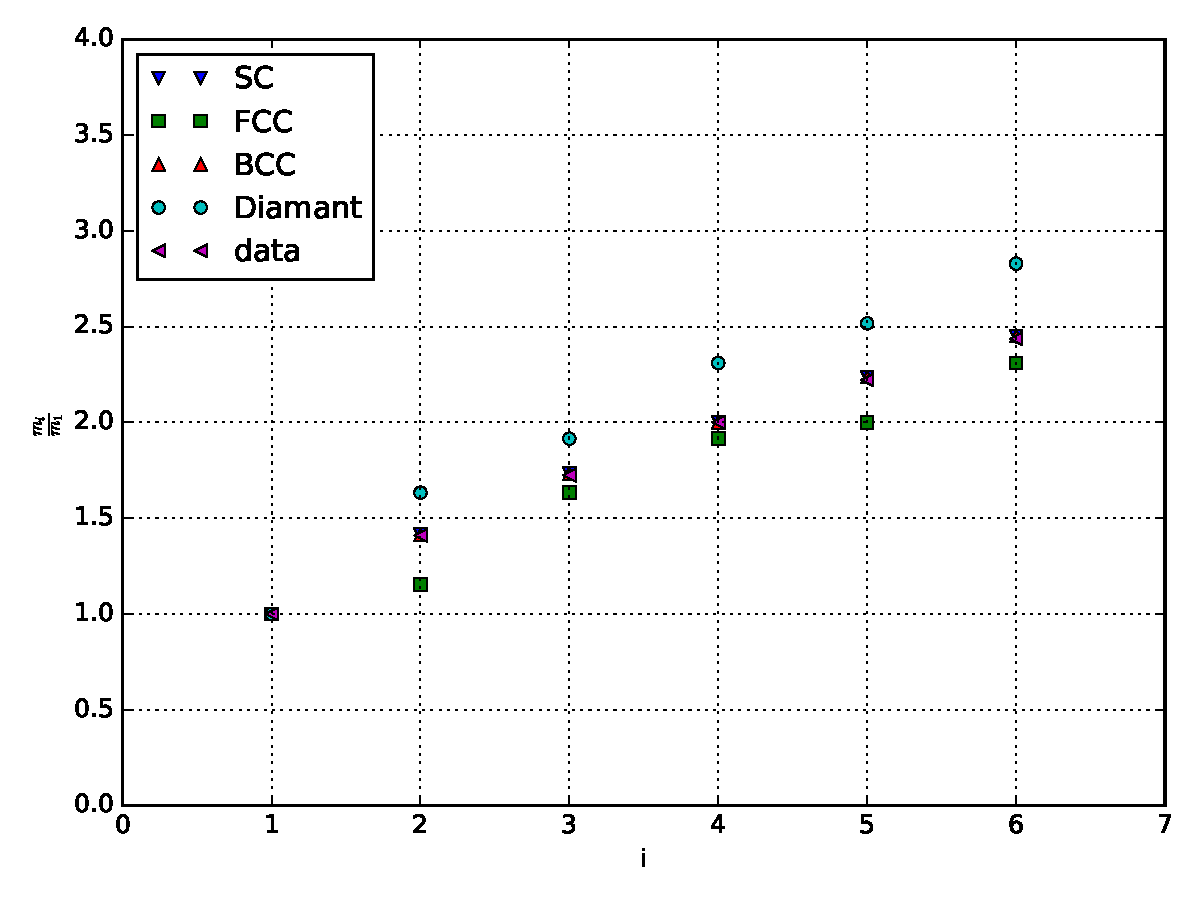
\includegraphics[width=\textwidth]{Abbildungen/verhaeltnisse.pdf}
		\subcaption{Verhältnisse $\frac{m_i}{m_1}$ für verschiedene Gittertypen und Daten für Metall.}
		\label{fig:verhaeltnisse_metall}
	\end{minipage}
	\begin{minipage}[t]{0.45\textwidth}
		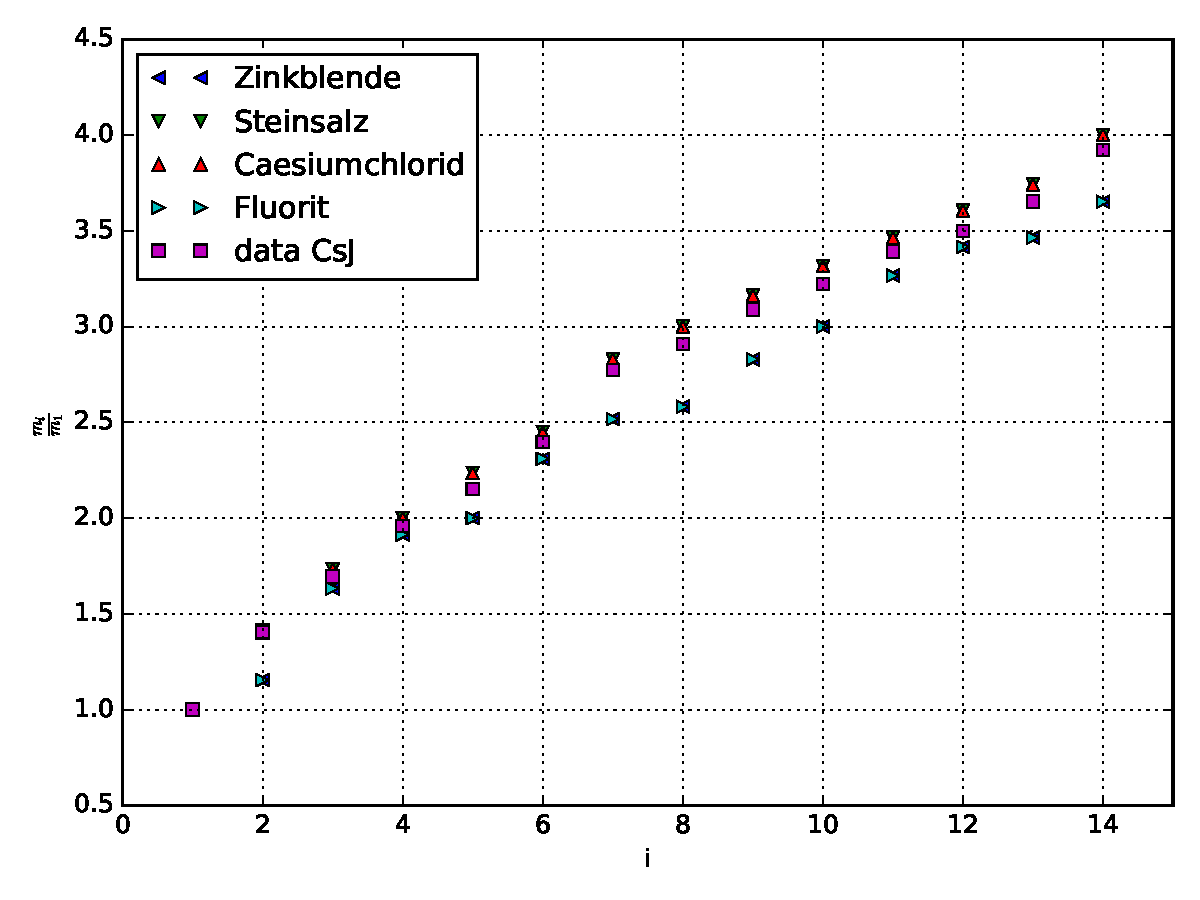
\includegraphics[width=\textwidth]{Abbildungen/verhaeltnisse_Salz.pdf}
		\subcaption{Verhältnisse $\frac{m_i}{m_1}$ für verschiedene Gittertypen und Daten für Salz.}
		\label{fig:verhaeltnisse_salz}
\end{minipage}
% \caption{Die Elementaren kubischen Gittertypen bei denen gilt $|a|=|b|= |c|$. \cite{Anleitung}}
\label{fig:verhaeltnisse}
\end{figure}
Da es nur drei Stoffe mit einer SC-Struktur gibt (Sauerstoff, Fluor und Polonium) ist bei dem Metall-Pulver von einer BCC-Struktur auszugehen. Für Salz wurde das gleiche Prozedere benutzt, nur dass diesmal die Formfaktoren, in Abbildung \ref{fig:formfaktoren} zu sehen, berücksichtigt werden müssen. Das bedeutet, dass für jede Struktur (Zinkblende-, Steinsalz-, Caesiumchlorid- und Fluoritstruktur) jede mögliche Kombination der Ionen, die in Abbildung \ref{fig:formfaktoren} zu sehen sind, getestet werden muss. Die theoretischen Verhältnisse $m_i / m_1$ geplottet gegen die Daten von Caesiumiodid (CsJ) sind in Abbildung \ref{fig:verhaeltnisse_salz} zu sehen. CsJ in der Caesiumchlorid-Sturktur ist der Stoff, der die kleinste Abweichung hat. 
% Die Abweichungen für jede Kombination sind in Tabelle \ref zu sehen.
\begin{figure}[h]
\centering
	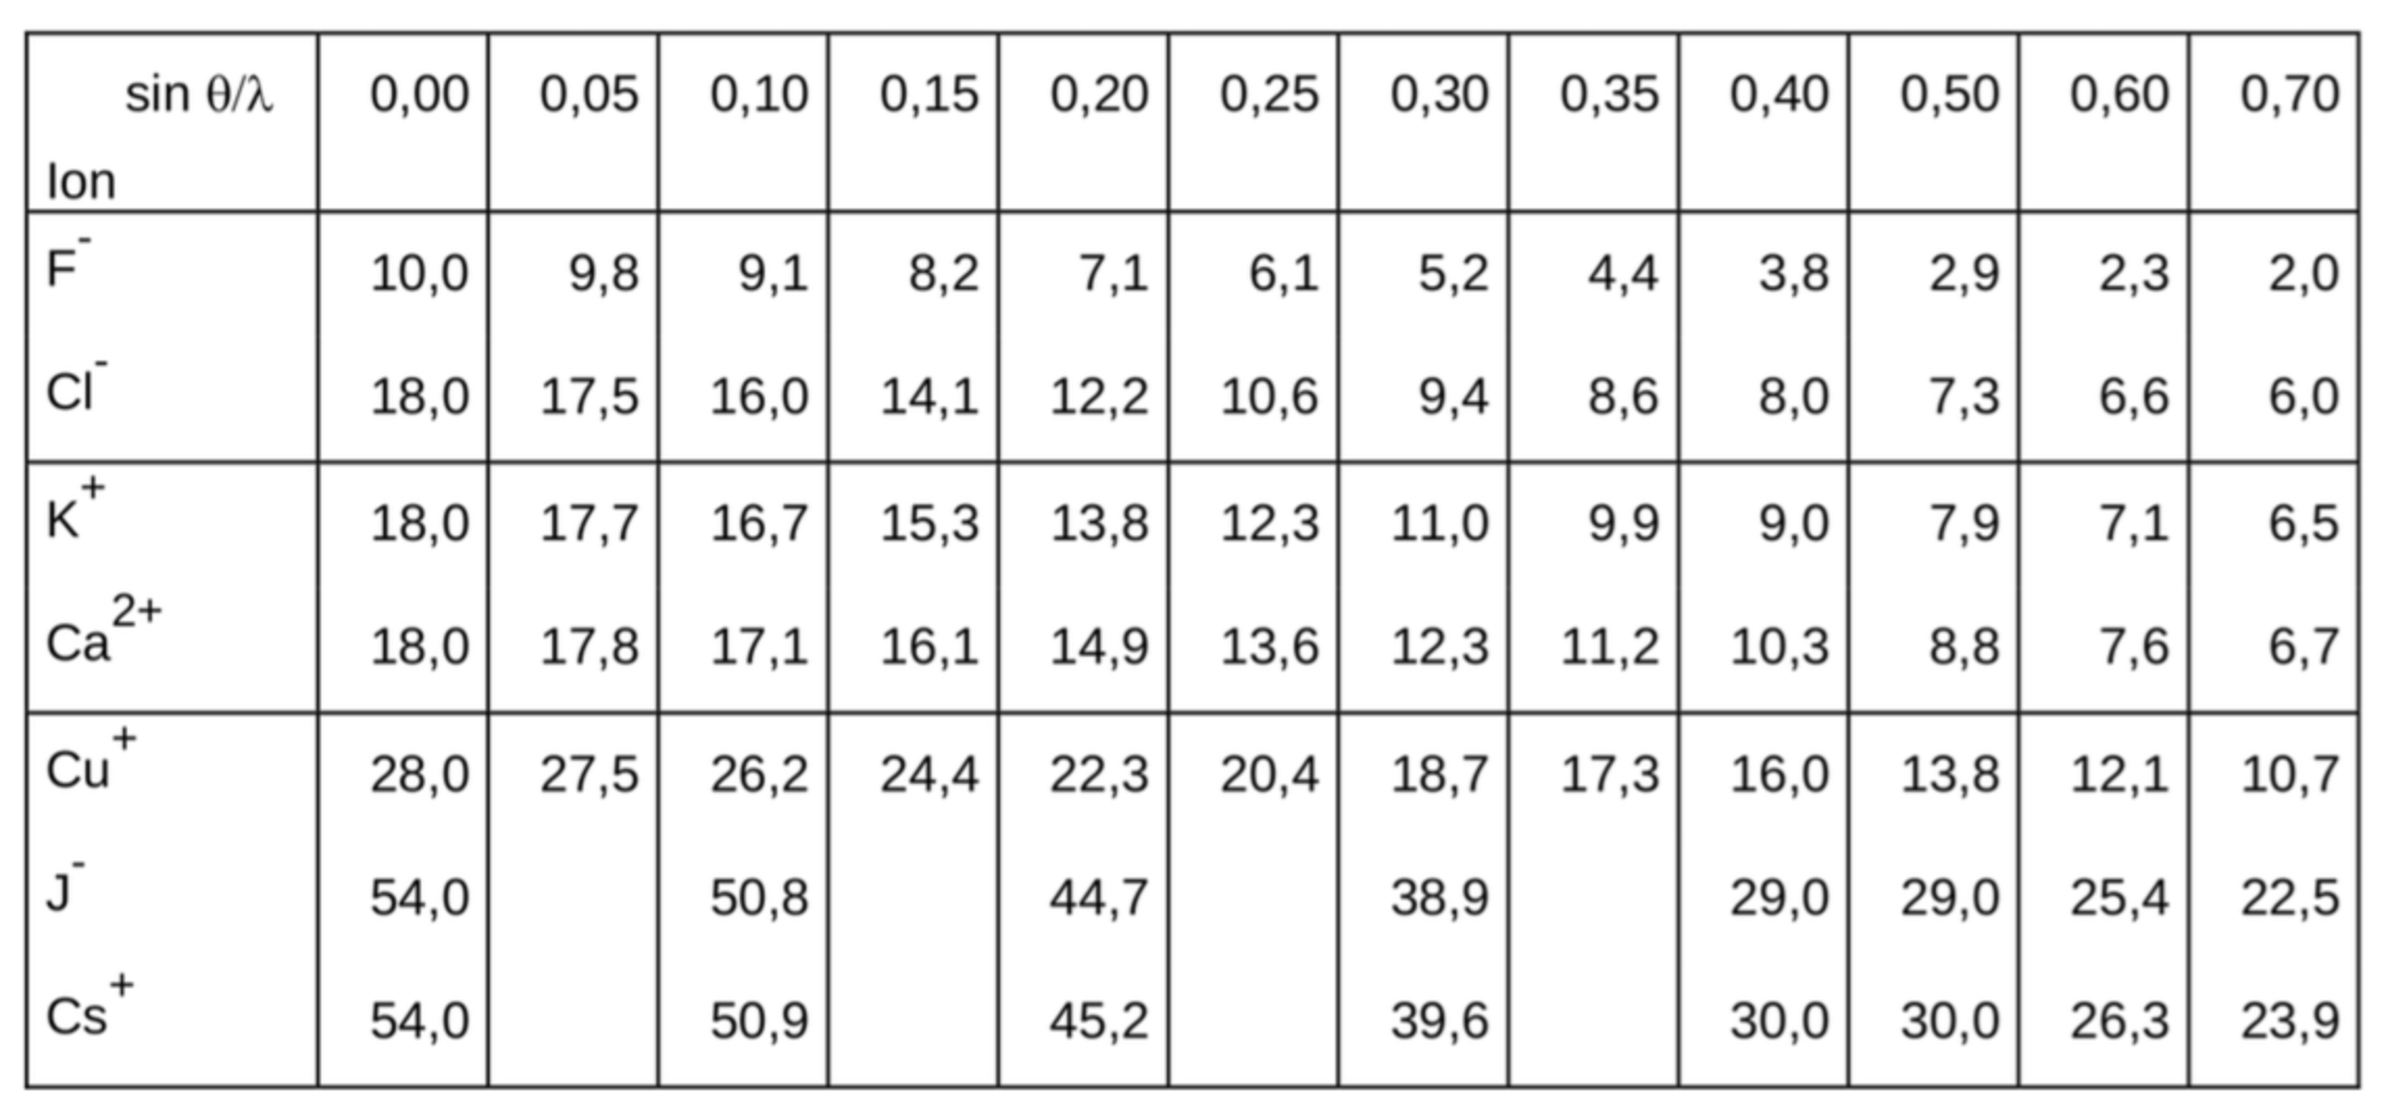
\includegraphics[width = 0.9\textwidth]{Abbildungen/formfaktoren.pdf}
\caption{Die Formfaktoren für verschiedene Ionen, je nach Winkel \cite{Anleitung}.}
\label{fig:formfaktoren}
\end{figure}

\subsection{Systematische Fehler}

Als Erstes ist darauf hinzuweisen, dass durch den Versuchsaufbau zwei systematische Fehler gemacht werden, die wie folgt in die Auswertung einfließen.
Die Systematischen Fehler entstehen bei den Ringradien. 
Dabei entsteht der Eindruck, dass die Gitterkonstante a abhängig von dem Beugungswinkel $\theta$ ist. \\
Der erste systematische Fehler liegt in der Messung von dem 4 $\theta$-Winkel, der stets zu groß gemessen wird. 
Problematisch ist das so kleine Winkel große Fehler besitzen. 
in Abbildung \ref{fig:sys1} wird schematisch gezeigt, wie das wahre $\theta$ aussehen sollte.
\begin{figure}
\centering
	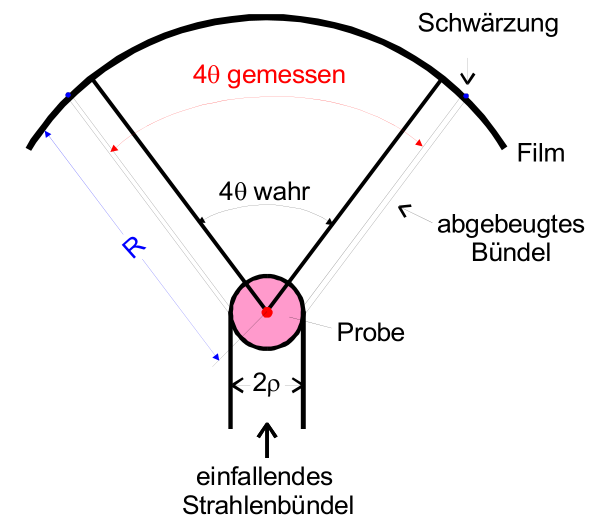
\includegraphics[width = 0.5\textwidth]{Abbildungen/Syst1.png}
	\caption{Darstellung des systematischen Fehlers, der aus der Absorbtion innerhalb des Probenstäbchens entsteht \cite{Anleitung}.}
	\label{fig:sys1}
\end{figure} 
Das Problem liegt darin, dass der Großteil der Strahlung komplett absorbiert wird und nur am Rand Beugungseffekte entstehen die aus der Probe kommen.
Berücksichtigt wird dies durch die Korrektur $\Delta a_A$ nach Bradley und Jay in Gleichung \ref{eq:syst1}.
\begin{equation}
\frac{\Delta a_A}{\text{a}} = \frac{\rho}{2\text{R}}\left( 1-\frac{\text{R}}{\text{F}} \right)\frac{\cos^2{\theta}}{\theta}
\label{eq:syst1}
\end{equation}
Der Größen sind in der Abbildung \ref{fig:sys1} dargestellt. 
$\rho$ ist der Radius des Probenstäbchens, R der Kameraradius und F der Abstand zwischen Fokus und Probe.
Dieser Fehler führt in dem Plot von $a(\theta)$ gegen $\cos^2{\theta}$ zu den Fehlerbalken in a.
\\\\
Der Zweite Systematische Fehler resultiert aus der Geometrie des Aufbaus.
In der Regel sind die Achse des Probenzylinders und die Achse des Films leicht gegeneinander verschoben. 
Das ist in Abbildung \ref{fig:sys2} dargestellt.
\begin{figure}
\centering
	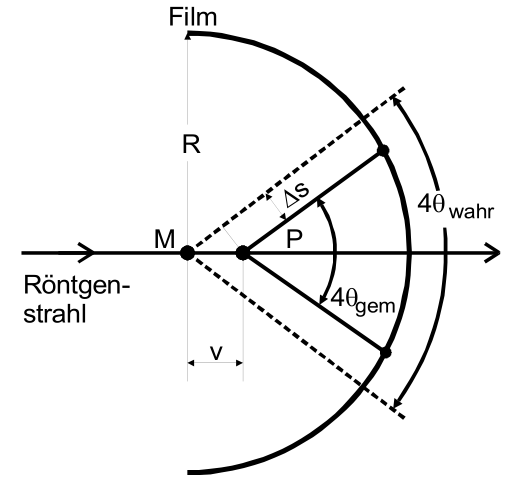
\includegraphics[width = 0.5\textwidth]{Abbildungen/Syst2.png}
	\caption{\cite{Anleitung}.}
	\label{fig:sys2}
\end{figure}
Dieser Fehler wirkt sich wieder auf das gemessene $\theta$ aus und ergibt die Abweichung $\Delta \theta$ wie in Gleichung \ref{eq:syst2} aufgeführt ist.
Der Abstand $\Delta$S und die Verschiebung v sind aus der Skizze \ref{fig:sys2} zu entnehmen.
\begin{align*}
\Delta \text{S} &  = -\text{v} \sin{2 \theta} \\
\Delta \theta & = -\frac{\Delta \text{S}}{2\text{R}}
\end{align*}
\begin{equation}
\Delta \theta = \frac{\text{v}}{2\text{R}}\sin{2\theta} = \frac{\text{v}}{\text{R}}\cos{\theta}\sin{\theta}
\label{eq:syst2}
\end{equation}
Unter Berücksichtigung der differnzierten Bragg-Bedingung ergibt sich der Korrekturterm $\Delta a_v$ in Gleichung \ref{eq:system} aus
\begin{align*}
\frac{\Delta \text{a}}{\text{a}} = \frac{\Delta \text{d}}{\text{d}} = -\Delta \theta \frac{\cos{\theta}}{\sin{\theta}}.
\end{align*}
\begin{equation}
\frac{\Delta a_v}{\text{a}} = \frac{\text{v}}{\text{R}}\cos^2{\theta}
\label{eq:system}
\end{equation}
Das heißt, die Gesamte Abweichung der Gitterkonstante resultiert in $\Delta a_{ges}$, welche as der Summe der beiden systematischen Fehler $\Delta a_A$ und $\Delta a_v$. 
Dabei ist die Gitterkonstante $\Delta a_{ges}$ proportional zu $\cos2{\theta}$.\\
Die tatsächliche Gitterkonstante a ist deshalb aus dem y-Achsenabschnitt des Plots $a(\theta)$ gegen $\cos^2{\theta}$ zu entnehmen.

<<<<<<< 3919e70f61e226b74a65735ba5c73a3a4af72710
\subsection{Metall}
||||||| merged common ancestors
ajwkhfkgWVUIwbefbbWJHEBFBHKJAEBKJFHWEHFVV
=======

\subsection{Metall}

ajwkhfkgWVUIwbefbbWJHEBFBHKJAEBKJFHWEHFVV
>>>>>>> Ein bisschen an der Auswertung getexet
=======
\subsection{Gitterkonstante}

Um den systematischen Fehler nach Gleichung (\ref{eq:system}) zu eliminieren und damit die Gitterkonstante zu bestimmen wird die Gitterkonstante $a$ gegen $\cos^2(\theta)$ geplottet und ein linearer Fit vollzogen. In Abbildung \ref{fig:fit_metall} ist der Fit für Metall zu sehen. In Abbildung \ref{fig:fit_salz} der Fit für Salz. Für Metall ergibt sich eine Gitterkonstante von $a_{metall} = \SI{2.86(18)e-10}{m}$, welche ziemlich genau mit dem Literaturwert von $a_{metall}^{lit} = \SI{2.86e-10}{m}$ \cite{metall} übereinstimmt. In Abbildung \ref{fig:fit_salz} ist der Fit für die Salz-Struktur zu sehen. Es wurde bereits durch die Strukturanalyse CsJ vorhergesagt. Der Fit liefert eine Gitterkonstante von $a_{salz} = \SI{4.48(20)e-10}{m}$ welche gut mit dem Literaturwert von $a_{salz}^{lit} = \SI{4.57e-10}{m}$ \cite{Gross} übereinstimmt.

\begin{figure}[h]
	\begin{minipage}[t]{0.45\textwidth}
		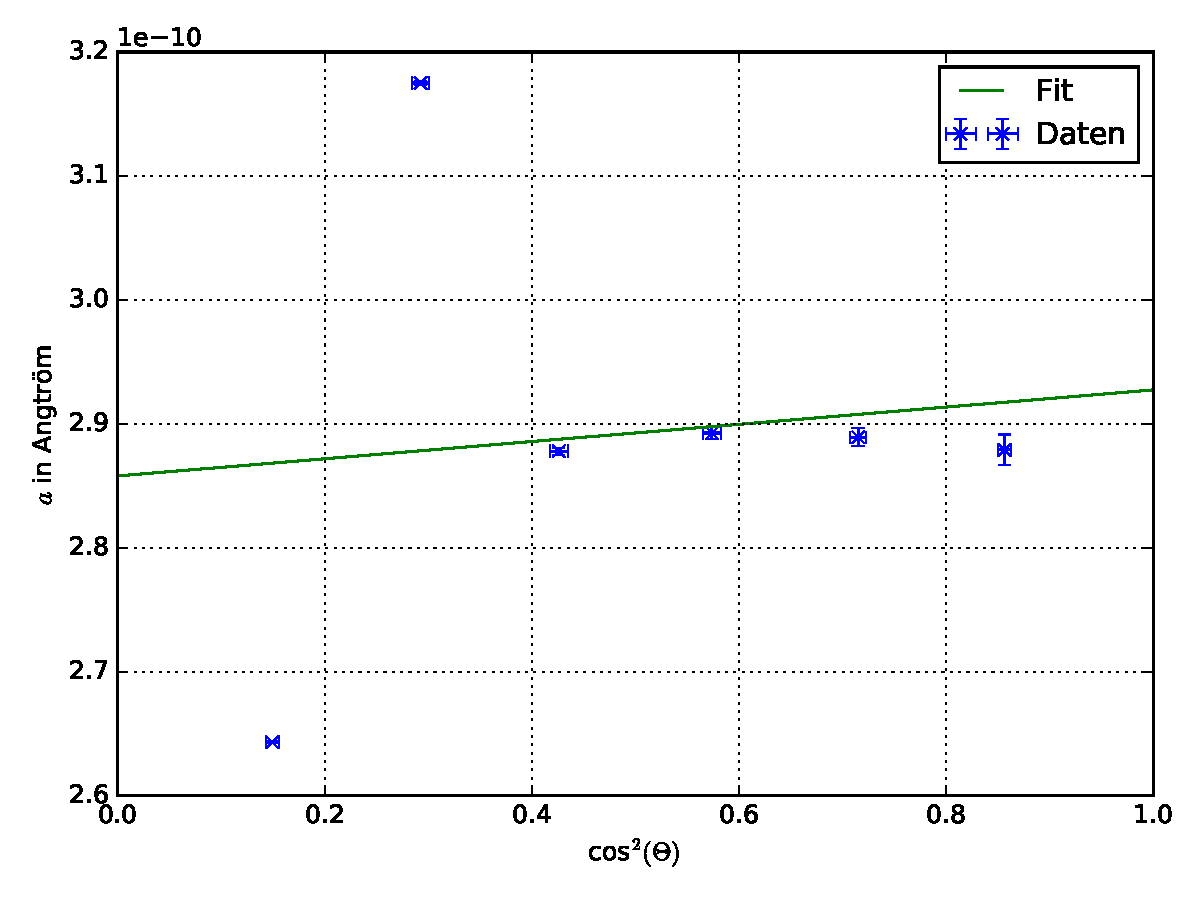
\includegraphics[width=\textwidth]{Abbildungen/Metall_Fit.pdf}
		\subcaption{Linearer Fit der Metall-Analyse um den systematischen Fehler durch die Verschiebung der Kristalle von der Achse zu eliminieren.}
		\label{fig:fit_metall}
	\end{minipage}
	\begin{minipage}[t]{0.45\textwidth}
		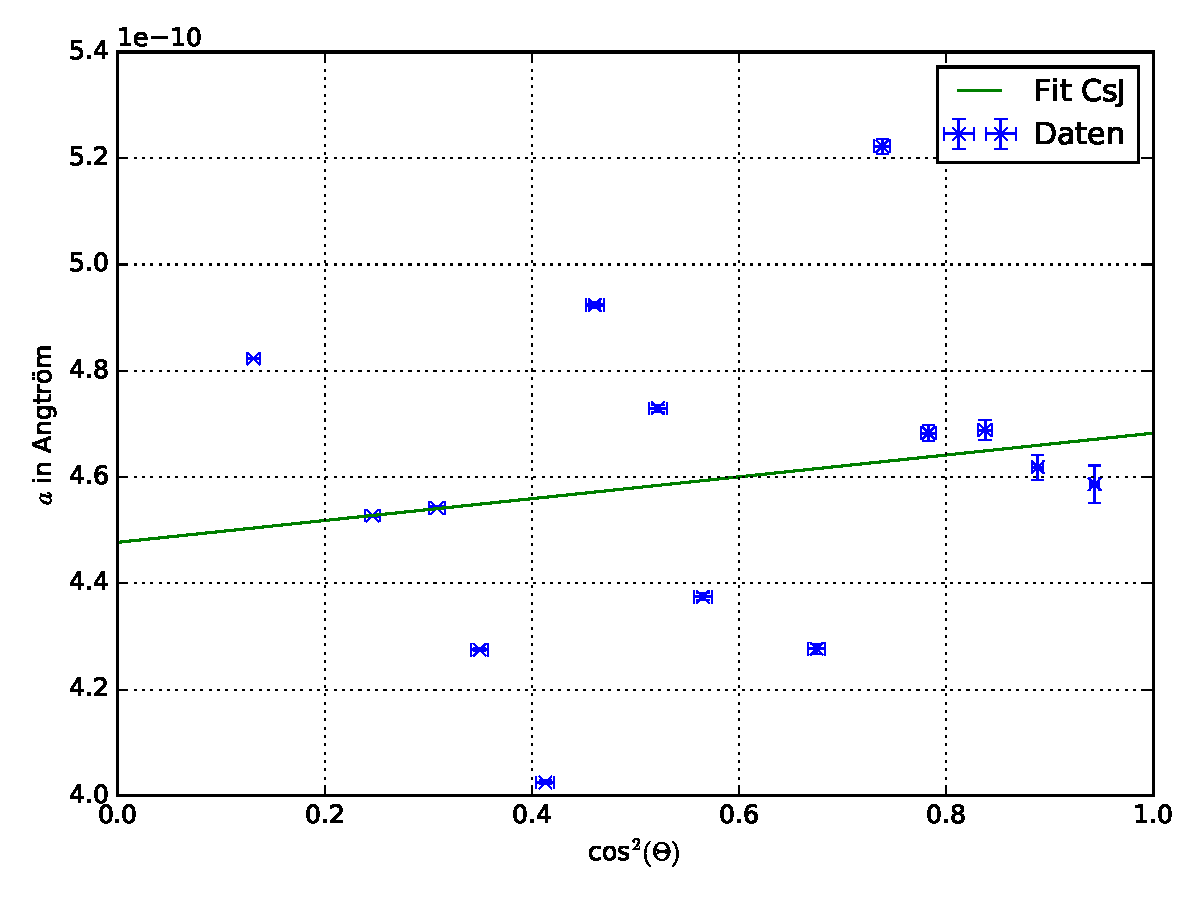
\includegraphics[width=\textwidth]{Abbildungen/Salz_Fit_Egor.pdf}
		\subcaption{Linearer Fit der Salz-Analyse um den systematischen Fehler durch die Verschiebung der Kristalle von der Achse zu eliminieren.}
		\label{fig:fit_salz}
\end{minipage}
% \caption{Die Elementaren kubischen Gittertypen bei denen gilt $|a|=|b|= |c|$. \cite{Anleitung}}
\end{figure}
>>>>>>> fürs erste fertig
